\documentclass[]{article}
\usepackage{lmodern}
\usepackage{amssymb,amsmath}
\usepackage{ifxetex,ifluatex}
\usepackage{fixltx2e} % provides \textsubscript
\ifnum 0\ifxetex 1\fi\ifluatex 1\fi=0 % if pdftex
  \usepackage[T1]{fontenc}
  \usepackage[utf8]{inputenc}
\else % if luatex or xelatex
  \ifxetex
    \usepackage{mathspec}
  \else
    \usepackage{fontspec}
  \fi
  \defaultfontfeatures{Ligatures=TeX,Scale=MatchLowercase}
\fi
% use upquote if available, for straight quotes in verbatim environments
\IfFileExists{upquote.sty}{\usepackage{upquote}}{}
% use microtype if available
\IfFileExists{microtype.sty}{%
\usepackage{microtype}
\UseMicrotypeSet[protrusion]{basicmath} % disable protrusion for tt fonts
}{}
\usepackage[margin=1in]{geometry}
\usepackage{hyperref}
\hypersetup{unicode=true,
            pdftitle={Mini Project: Unsupervised Learning Analysis of Cancer Cells},
            pdfborder={0 0 0},
            breaklinks=true}
\urlstyle{same}  % don't use monospace font for urls
\usepackage{color}
\usepackage{fancyvrb}
\newcommand{\VerbBar}{|}
\newcommand{\VERB}{\Verb[commandchars=\\\{\}]}
\DefineVerbatimEnvironment{Highlighting}{Verbatim}{commandchars=\\\{\}}
% Add ',fontsize=\small' for more characters per line
\usepackage{framed}
\definecolor{shadecolor}{RGB}{248,248,248}
\newenvironment{Shaded}{\begin{snugshade}}{\end{snugshade}}
\newcommand{\KeywordTok}[1]{\textcolor[rgb]{0.13,0.29,0.53}{\textbf{#1}}}
\newcommand{\DataTypeTok}[1]{\textcolor[rgb]{0.13,0.29,0.53}{#1}}
\newcommand{\DecValTok}[1]{\textcolor[rgb]{0.00,0.00,0.81}{#1}}
\newcommand{\BaseNTok}[1]{\textcolor[rgb]{0.00,0.00,0.81}{#1}}
\newcommand{\FloatTok}[1]{\textcolor[rgb]{0.00,0.00,0.81}{#1}}
\newcommand{\ConstantTok}[1]{\textcolor[rgb]{0.00,0.00,0.00}{#1}}
\newcommand{\CharTok}[1]{\textcolor[rgb]{0.31,0.60,0.02}{#1}}
\newcommand{\SpecialCharTok}[1]{\textcolor[rgb]{0.00,0.00,0.00}{#1}}
\newcommand{\StringTok}[1]{\textcolor[rgb]{0.31,0.60,0.02}{#1}}
\newcommand{\VerbatimStringTok}[1]{\textcolor[rgb]{0.31,0.60,0.02}{#1}}
\newcommand{\SpecialStringTok}[1]{\textcolor[rgb]{0.31,0.60,0.02}{#1}}
\newcommand{\ImportTok}[1]{#1}
\newcommand{\CommentTok}[1]{\textcolor[rgb]{0.56,0.35,0.01}{\textit{#1}}}
\newcommand{\DocumentationTok}[1]{\textcolor[rgb]{0.56,0.35,0.01}{\textbf{\textit{#1}}}}
\newcommand{\AnnotationTok}[1]{\textcolor[rgb]{0.56,0.35,0.01}{\textbf{\textit{#1}}}}
\newcommand{\CommentVarTok}[1]{\textcolor[rgb]{0.56,0.35,0.01}{\textbf{\textit{#1}}}}
\newcommand{\OtherTok}[1]{\textcolor[rgb]{0.56,0.35,0.01}{#1}}
\newcommand{\FunctionTok}[1]{\textcolor[rgb]{0.00,0.00,0.00}{#1}}
\newcommand{\VariableTok}[1]{\textcolor[rgb]{0.00,0.00,0.00}{#1}}
\newcommand{\ControlFlowTok}[1]{\textcolor[rgb]{0.13,0.29,0.53}{\textbf{#1}}}
\newcommand{\OperatorTok}[1]{\textcolor[rgb]{0.81,0.36,0.00}{\textbf{#1}}}
\newcommand{\BuiltInTok}[1]{#1}
\newcommand{\ExtensionTok}[1]{#1}
\newcommand{\PreprocessorTok}[1]{\textcolor[rgb]{0.56,0.35,0.01}{\textit{#1}}}
\newcommand{\AttributeTok}[1]{\textcolor[rgb]{0.77,0.63,0.00}{#1}}
\newcommand{\RegionMarkerTok}[1]{#1}
\newcommand{\InformationTok}[1]{\textcolor[rgb]{0.56,0.35,0.01}{\textbf{\textit{#1}}}}
\newcommand{\WarningTok}[1]{\textcolor[rgb]{0.56,0.35,0.01}{\textbf{\textit{#1}}}}
\newcommand{\AlertTok}[1]{\textcolor[rgb]{0.94,0.16,0.16}{#1}}
\newcommand{\ErrorTok}[1]{\textcolor[rgb]{0.64,0.00,0.00}{\textbf{#1}}}
\newcommand{\NormalTok}[1]{#1}
\usepackage{graphicx,grffile}
\makeatletter
\def\maxwidth{\ifdim\Gin@nat@width>\linewidth\linewidth\else\Gin@nat@width\fi}
\def\maxheight{\ifdim\Gin@nat@height>\textheight\textheight\else\Gin@nat@height\fi}
\makeatother
% Scale images if necessary, so that they will not overflow the page
% margins by default, and it is still possible to overwrite the defaults
% using explicit options in \includegraphics[width, height, ...]{}
\setkeys{Gin}{width=\maxwidth,height=\maxheight,keepaspectratio}
\IfFileExists{parskip.sty}{%
\usepackage{parskip}
}{% else
\setlength{\parindent}{0pt}
\setlength{\parskip}{6pt plus 2pt minus 1pt}
}
\setlength{\emergencystretch}{3em}  % prevent overfull lines
\providecommand{\tightlist}{%
  \setlength{\itemsep}{0pt}\setlength{\parskip}{0pt}}
\setcounter{secnumdepth}{0}
% Redefines (sub)paragraphs to behave more like sections
\ifx\paragraph\undefined\else
\let\oldparagraph\paragraph
\renewcommand{\paragraph}[1]{\oldparagraph{#1}\mbox{}}
\fi
\ifx\subparagraph\undefined\else
\let\oldsubparagraph\subparagraph
\renewcommand{\subparagraph}[1]{\oldsubparagraph{#1}\mbox{}}
\fi

%%% Use protect on footnotes to avoid problems with footnotes in titles
\let\rmarkdownfootnote\footnote%
\def\footnote{\protect\rmarkdownfootnote}

%%% Change title format to be more compact
\usepackage{titling}

% Create subtitle command for use in maketitle
\newcommand{\subtitle}[1]{
  \posttitle{
    \begin{center}\large#1\end{center}
    }
}

\setlength{\droptitle}{-2em}
  \title{Mini Project: Unsupervised Learning Analysis of Cancer Cells}
  \pretitle{\vspace{\droptitle}\centering\huge}
  \posttitle{\par}
  \author{}
  \preauthor{}\postauthor{}
  \date{}
  \predate{}\postdate{}


\begin{document}
\maketitle

\subsection{Background}\label{background}

The goal of this hands-on session is for you to explore a complete
analysis using the unsupervised learning techniques covered in the last
class. You'll extend what you've learned by combining PCA as a
preprocessing step to clustering using data that consist of measurements
of cell nuclei of human breast masses. This expands on our RNA-Seq
analysis from last day.

The data itself comes from the \emph{Wisconsin Breast Cancer Diagnostic
Data Set} first reported by
\href{http://archive.ics.uci.edu/ml/datasets/Breast+Cancer+Wisconsin+\%2528Diagnostic\%2529}{\emph{K.
P. Benne and O. L. Mangasarian: ``Robust Linear Programming
Discrimination of Two Linearly Inseparable Sets''}}.

Values in this data set describe characteristics of the cell nuclei
present in digitized images of a fine needle aspiration (FNA) of a
breast mass. For example \texttt{radius} (i.e.~mean of distances from
center to points on the perimeter), \texttt{texture} (i.e.~standard
deviation of gray-scale values), and \texttt{smoothness} (local
variation in radius lengths). Summary information is also provided for
each group of cells including \texttt{diagnosis} (i.e.~benign (not
cancerous) and and malignant (cancerous)).

\section{Section 1.}\label{section-1.}

\subsection{Preparing the data}\label{preparing-the-data}

Before we can begin our analysis we first have to download and import
our data correctly into our R session.

For this we can use the \texttt{read.csv()} function to read the CSV
(comma-separated values) file containing the data from the URL:
\url{https://bioboot.github.io/bimm143_W18/class-material/WisconsinCancer.csv}

Assign the result to an object called \texttt{wisc.df}.

\begin{Shaded}
\begin{Highlighting}[]
\NormalTok{url <-}\StringTok{ "https://bioboot.github.io/bimm143_W18/class-material/WisconsinCancer.csv"}

\CommentTok{# Complete the following code to input the data and store as wisc.df}
\NormalTok{wisc.df <-}\StringTok{ }\NormalTok{___}
\end{Highlighting}
\end{Shaded}

Examine your input data to ensure column names are set correctly. The
\texttt{id} and \texttt{diagnosis} columns will not be used for most of
the following steps. Use \texttt{as.matrix()} to convert the other
features (i.e.~columns) of the data (in columns 3 through 32) to a
matrix. Store this in a variable called \texttt{wisc.data}.

\begin{Shaded}
\begin{Highlighting}[]
\CommentTok{# Convert the features of the data: wisc.data}
\NormalTok{wisc.data <-}\StringTok{ }\KeywordTok{as.matrix}\NormalTok{( ___ )}
\end{Highlighting}
\end{Shaded}

Assign the row names of \texttt{wisc.data} the values currently
contained in the \texttt{id} column of \texttt{wisc.df}. While not
strictly required, this will help you keep track of the different
observations throughout the modeling process.

\begin{Shaded}
\begin{Highlighting}[]
\CommentTok{# Set the row names of wisc.data}
\KeywordTok{row.names}\NormalTok{(wisc.data) <-}\StringTok{ }\NormalTok{wisc.df}\OperatorTok{$}\NormalTok{id}
\CommentTok{#head(wisc.data)}
\end{Highlighting}
\end{Shaded}

Finally, setup a separate new vector called \texttt{diagnosis} to be
\texttt{1} if a diagnosis is malignant (\texttt{"M"}) and \texttt{0}
otherwise. Note that R coerces \texttt{TRUE} to \texttt{1} and
\texttt{FALSE} to \texttt{0}.

\begin{Shaded}
\begin{Highlighting}[]
\CommentTok{# Create diagnosis vector by completing the missing code}
\NormalTok{diagnosis <-}\StringTok{ }\KeywordTok{as.numeric}\NormalTok{( ___ )}
\end{Highlighting}
\end{Shaded}

\subsection{Exploratory data analysis}\label{exploratory-data-analysis}

The first step of any data analysis, unsupervised or supervised, is to
familiarize yourself with the data.

Explore the data you created before (\texttt{wisc.data} and
\texttt{diagnosis}) to answer the following questions:

\begin{itemize}
\tightlist
\item
  \textbf{Q1}. How many observations are in this dataset?
\item
  \textbf{Q2}. How many variables/features in the data are suffixed with
  \texttt{\_mean}?
\item
  \textbf{Q3}. How many of the observations have a malignant diagnosis?
\end{itemize}

\begin{quote}
The functions \texttt{dim()}, \texttt{length()}, \texttt{grep()} and
\texttt{sum()} may be useful for answering the first 3 questions above.
\end{quote}

\section{Section 2.}\label{section-2.}

\subsection{Performing PCA}\label{performing-pca}

The next step in your analysis is to perform principal component
analysis (PCA) on \texttt{wisc.data}.

It is important to check if the data need to be scaled before performing
PCA. Recall two common reasons for scaling data include:

\begin{itemize}
\tightlist
\item
  The input variables use different units of measurement.
\item
  The input variables have significantly different variances.
\end{itemize}

Check the mean and standard deviation of the features (i.e.~columns) of
the \texttt{wisc.data} to determine if the data should be scaled. Use
the \texttt{colMeans()} and \texttt{apply()} functions like you've done
before.

\begin{Shaded}
\begin{Highlighting}[]
\CommentTok{# Check column means and standard deviations}
\KeywordTok{colMeans}\NormalTok{(wisc.data)}

\KeywordTok{apply}\NormalTok{(wisc.data,}\DecValTok{2}\NormalTok{,sd)}
\end{Highlighting}
\end{Shaded}

Execute PCA with the \texttt{prcomp()} function on the
\texttt{wisc.data}, scaling if appropriate, and assign the output model
to \texttt{wisc.pr}.

\begin{Shaded}
\begin{Highlighting}[]
\CommentTok{# Perform PCA on wisc.data by completing the following code}
\NormalTok{wisc.pr <-}\StringTok{ }\KeywordTok{prcomp}\NormalTok{( ___ )}
\end{Highlighting}
\end{Shaded}

Inspect a summary of the results with the \texttt{summary()} function.

\begin{Shaded}
\begin{Highlighting}[]
\CommentTok{# Look at summary of results}
\KeywordTok{summary}\NormalTok{(wisc.pr)}
\end{Highlighting}
\end{Shaded}

\begin{verbatim}
## Importance of components%s:
##                           PC1    PC2     PC3     PC4     PC5     PC6
## Standard deviation     3.6444 2.3857 1.67867 1.40735 1.28403 1.09880
## Proportion of Variance 0.4427 0.1897 0.09393 0.06602 0.05496 0.04025
## Cumulative Proportion  0.4427 0.6324 0.72636 0.79239 0.84734 0.88759
##                            PC7     PC8    PC9    PC10   PC11    PC12
## Standard deviation     0.82172 0.69037 0.6457 0.59219 0.5421 0.51104
## Proportion of Variance 0.02251 0.01589 0.0139 0.01169 0.0098 0.00871
## Cumulative Proportion  0.91010 0.92598 0.9399 0.95157 0.9614 0.97007
##                           PC13    PC14    PC15    PC16    PC17    PC18
## Standard deviation     0.49128 0.39624 0.30681 0.28260 0.24372 0.22939
## Proportion of Variance 0.00805 0.00523 0.00314 0.00266 0.00198 0.00175
## Cumulative Proportion  0.97812 0.98335 0.98649 0.98915 0.99113 0.99288
##                           PC19    PC20   PC21    PC22    PC23   PC24
## Standard deviation     0.22244 0.17652 0.1731 0.16565 0.15602 0.1344
## Proportion of Variance 0.00165 0.00104 0.0010 0.00091 0.00081 0.0006
## Cumulative Proportion  0.99453 0.99557 0.9966 0.99749 0.99830 0.9989
##                           PC25    PC26    PC27    PC28    PC29    PC30
## Standard deviation     0.12442 0.09043 0.08307 0.03987 0.02736 0.01153
## Proportion of Variance 0.00052 0.00027 0.00023 0.00005 0.00002 0.00000
## Cumulative Proportion  0.99942 0.99969 0.99992 0.99997 1.00000 1.00000
\end{verbatim}

\begin{itemize}
\tightlist
\item
  \textbf{Q4}. From your results, what proportion of the original
  variance is captured by the first principal components (PC1)?\\
\item
  \textbf{Q5}. How many principal components (PCs) are required to
  describe at least 70\% of the original variance in the data?
\item
  \textbf{Q6}. How many principal components (PCs) are required to
  describe at least 90\% of the original variance in the data?
\end{itemize}

\subsection{Interpreting PCA results}\label{interpreting-pca-results}

Now you will use some visualizations to better understand your PCA
model. You were introduced to one of these visualizations, the biplot,
last day.

You will often run into some common challenges with using biplots on
real-world data containing a non-trivial number of observations and
variables, then you'll look at some alternative visualizations. You are
encouraged to experiment with additional visualizations before moving on
to the next section

Create a biplot of the \texttt{wisc.pr} using the \texttt{biplot()}
function.

\begin{itemize}
\tightlist
\item
  \textbf{Q7.} What stands out to you about this plot? Is it easy or
  difficult to understand? Why?
\end{itemize}

\begin{Shaded}
\begin{Highlighting}[]
\KeywordTok{biplot}\NormalTok{(wisc.pr)}
\end{Highlighting}
\end{Shaded}

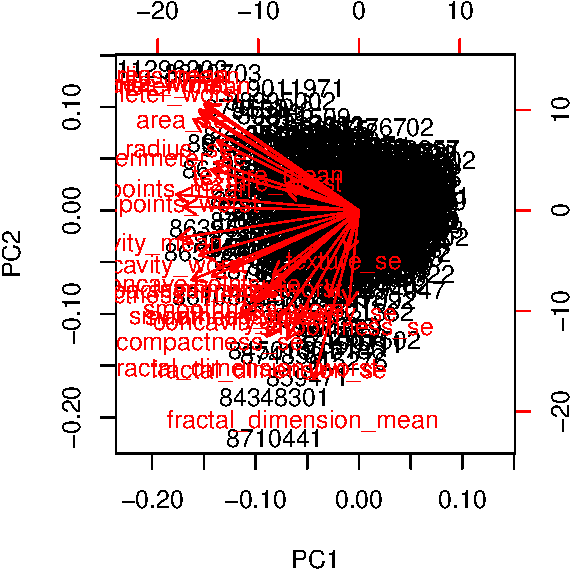
\includegraphics{lecture9_lab_files/figure-latex/unnamed-chunk-4-1.pdf}

Rownames are used as the plotting character for biplots like this one
which can make trends rather hard to see. Lets generate a more standard
scatter plot of each observation along principal components 1 and 2
(i.e.~a plot of PC1 vs PC2 available as the first two columns of
\texttt{wisc.pr\$x}) and color the points by the diagnosis (available in
the \texttt{diagnosis} vector you created earlier).

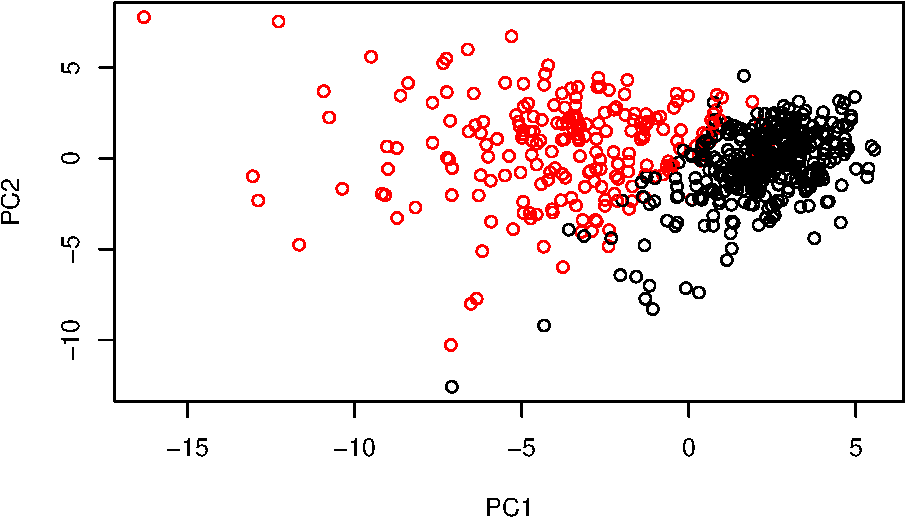
\includegraphics{lecture9_lab_files/figure-latex/unnamed-chunk-5-1.pdf}

\begin{Shaded}
\begin{Highlighting}[]
\CommentTok{# Scatter plot observations by components 1 and 2}
\KeywordTok{plot}\NormalTok{( ___ , }\DataTypeTok{col =}\NormalTok{ ___ , }
     \DataTypeTok{xlab =} \StringTok{"PC1"}\NormalTok{, }\DataTypeTok{ylab =} \StringTok{"PC2"}\NormalTok{)}
\end{Highlighting}
\end{Shaded}

\begin{itemize}
\tightlist
\item
  \textbf{Q8.} Repeat the same for principal components 1 and 3. What do
  you notice about these plots?
\end{itemize}

\begin{Shaded}
\begin{Highlighting}[]
\CommentTok{# Repeat for components 1 and 3}
\KeywordTok{plot}\NormalTok{(wisc.pr}\OperatorTok{$}\NormalTok{x[, }\KeywordTok{c}\NormalTok{(}\DecValTok{1}\NormalTok{, }\DecValTok{3}\NormalTok{)], }\DataTypeTok{col =}\NormalTok{ (diagnosis }\OperatorTok{+}\StringTok{ }\DecValTok{1}\NormalTok{), }
     \DataTypeTok{xlab =} \StringTok{"PC1"}\NormalTok{, }\DataTypeTok{ylab =} \StringTok{"PC3"}\NormalTok{)}
\end{Highlighting}
\end{Shaded}

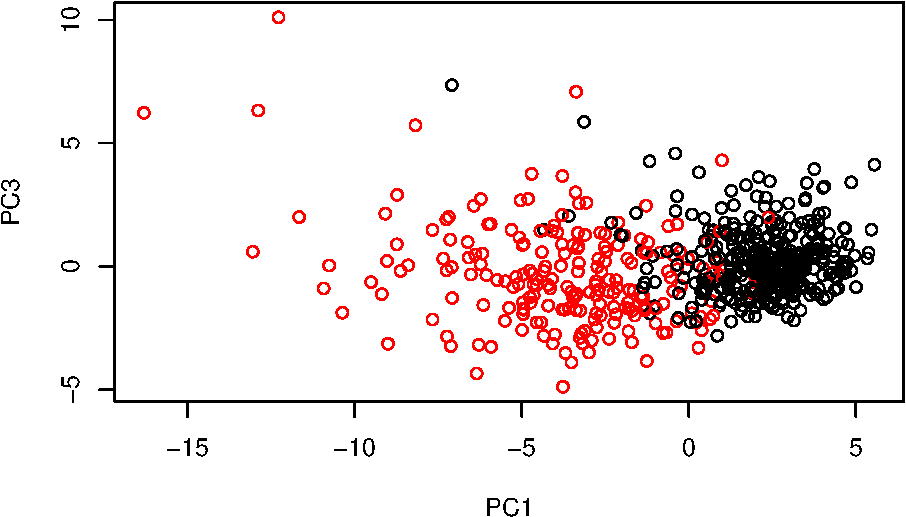
\includegraphics{lecture9_lab_files/figure-latex/unnamed-chunk-7-1.pdf}

\begin{Shaded}
\begin{Highlighting}[]
\CommentTok{# Do additional data exploration of your choosing below (optional)}
\end{Highlighting}
\end{Shaded}

Because principal component 2 explains more variance in the original
data than principal component 3, you can see that the first plot has a
cleaner cut separating the two subgroups.

\begin{quote}
Overall, the plots indicate that principal component 1 is capturing a
separation of malignant from benign samples. This is an important and
interesting result worthy of further exploration - as we will do in the
next sections!
\end{quote}

\subsection{Variance explained}\label{variance-explained}

In this exercise, you will produce scree plots showing the proportion of
variance explained as the number of principal components increases. The
data from PCA must be prepared for these plots, as there is not a
built-in function in base R to create them directly from the PCA model.

As you look at these plots, ask yourself if there's an `elbow' in the
amount of variance explained that might lead you to pick a natural
number of principal components. If an obvious elbow does not exist, as
is typical in some real-world datasets, consider how else you might
determine the number of principal components to retain based on the
scree plot.

Calculate the variance of each principal component by squaring the sdev
component of \texttt{wisc.pr} (i.e. \texttt{wisc.pr\$sdev\^{}2}). Save
the result as an object called \texttt{pr.var}.

Calculate the variance explained by each principal component by dividing
by the total variance explained of all principal components. Assign this
to a variable called \texttt{pve} and create a plot of variance
explained for each principal component.

\begin{Shaded}
\begin{Highlighting}[]
\CommentTok{# Variance explained by each principal component: pve}
\NormalTok{pve <-}\StringTok{ }\NormalTok{___ }\OperatorTok{/}\StringTok{ }\NormalTok{___}

\CommentTok{# Plot variance explained for each principal component}
\KeywordTok{plot}\NormalTok{(pve, }\DataTypeTok{xlab =} \StringTok{"Principal Component"}\NormalTok{, }
     \DataTypeTok{ylab =} \StringTok{"Proportion of Variance Explained"}\NormalTok{, }
     \DataTypeTok{ylim =} \KeywordTok{c}\NormalTok{(}\DecValTok{0}\NormalTok{, }\DecValTok{1}\NormalTok{), }\DataTypeTok{type =} \StringTok{"o"}\NormalTok{)}
\end{Highlighting}
\end{Shaded}

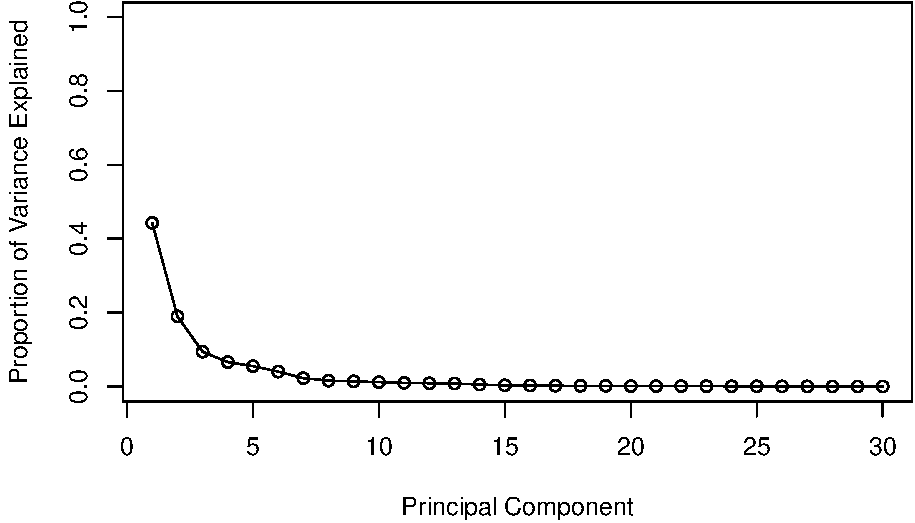
\includegraphics{lecture9_lab_files/figure-latex/var-1.pdf}

Using the \texttt{cumsum()} function, create a plot of cumulative
proportion of variance explained.

\begin{Shaded}
\begin{Highlighting}[]
\CommentTok{# Plot cumulative proportion of variance explained}
\KeywordTok{plot}\NormalTok{(}\KeywordTok{cumsum}\NormalTok{(pve), }\DataTypeTok{xlab =} \StringTok{"Principal Component"}\NormalTok{, }
     \DataTypeTok{ylab =} \StringTok{"Cumulative Proportion of Variance Explained"}\NormalTok{, }
     \DataTypeTok{ylim =} \KeywordTok{c}\NormalTok{(}\DecValTok{0}\NormalTok{, }\DecValTok{1}\NormalTok{), }\DataTypeTok{type =} \StringTok{"o"}\NormalTok{)}
\end{Highlighting}
\end{Shaded}

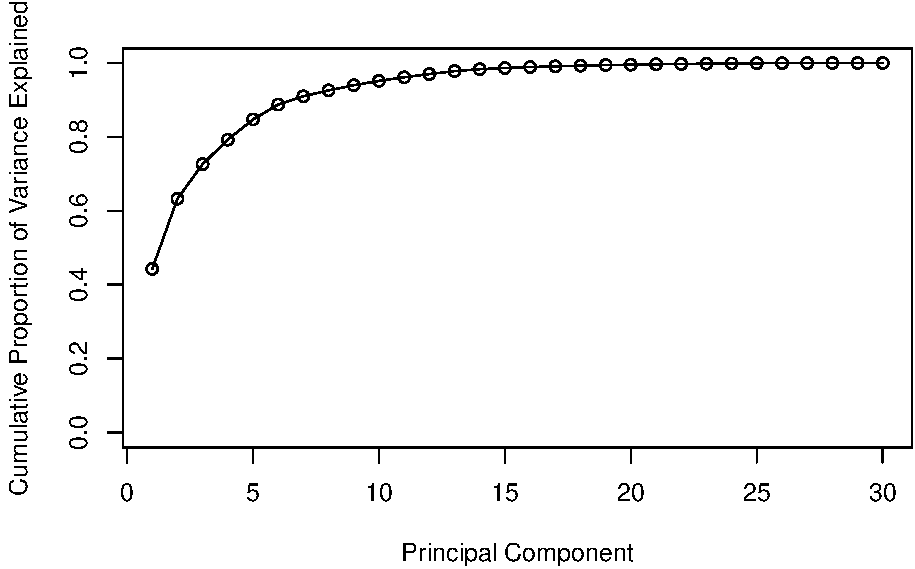
\includegraphics{lecture9_lab_files/figure-latex/cumsum-1.pdf}

\begin{Shaded}
\begin{Highlighting}[]
\CommentTok{# Plot cumulative proportion of variance explained}
\KeywordTok{plot}\NormalTok{( ___ , }\DataTypeTok{xlab =} \StringTok{"Principal Component"}\NormalTok{, }
     \DataTypeTok{ylab =} \StringTok{"Cumulative Proportion of Variance Explained"}\NormalTok{, }
     \DataTypeTok{ylim =} \KeywordTok{c}\NormalTok{(}\DecValTok{0}\NormalTok{, }\DecValTok{1}\NormalTok{), }\DataTypeTok{type =} \StringTok{"o"}\NormalTok{)}
\end{Highlighting}
\end{Shaded}

Use the \texttt{par()} function to create a side by side plot (i.e.~1
row 2 column arrangement) of these two graphs.

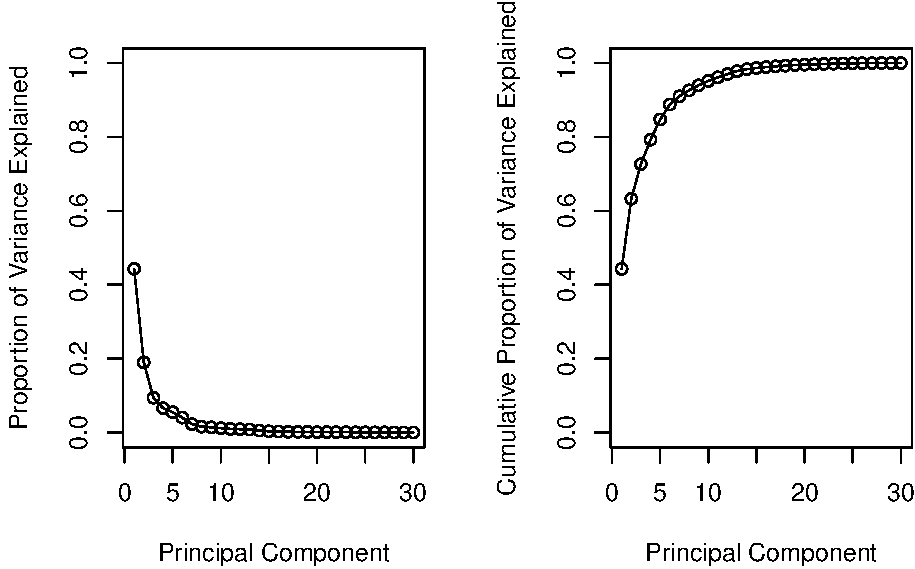
\includegraphics{lecture9_lab_files/figure-latex/unnamed-chunk-10-1.pdf}

\subsection{Communicating PCA results}\label{communicating-pca-results}

In this section we will check your understanding of the PCA results, in
particular the loadings and variance explained. The loadings,
represented as vectors, explain the mapping from the original features
to the principal components. The principal components are naturally
ordered from the most variance explained to the least variance
explained.

\begin{itemize}
\item
  \textbf{Q9.} For the first principal component, what is the component
  of the loading vector (i.e. \texttt{wisc.pr\$rotation{[},1{]}}) for
  the feature \texttt{concave.points\_mean}?
\item
  \textbf{Q10.} What is the minimum number of principal components
  required to explain 80\% of the variance of the data?
\end{itemize}

\section{Section 3.}\label{section-3.}

\subsection{Hierarchical clustering of case
data}\label{hierarchical-clustering-of-case-data}

The goal of this section is to do hierarchical clustering of the
observations. Recall from our last class that this type of clustering
does not assume in advance the number of natural groups that exist in
the data.

As part of the preparation for hierarchical clustering, the distance
between all pairs of observations are computed. Furthermore, there are
different ways to link clusters together, with single, complete, and
average being the most common linkage methods.

Scale the \texttt{wisc.data} data and assign the result to
\texttt{data.scaled}.

\begin{Shaded}
\begin{Highlighting}[]
\CommentTok{# Scale the wisc.data data: data.scaled}
\NormalTok{data.scaled <-}\StringTok{ }\KeywordTok{___}\NormalTok{(wisc.data)}
\end{Highlighting}
\end{Shaded}

Calculate the (Euclidean) distances between all pairs of observations in
the new scaled dataset and assign the result to \texttt{data.dist}.

\begin{Shaded}
\begin{Highlighting}[]
\NormalTok{data.dist <-}\StringTok{ }\KeywordTok{___}\NormalTok{(data.scaled)}
\end{Highlighting}
\end{Shaded}

Create a hierarchical clustering model using complete linkage. Manually
specify the method argument to hclust() and assign the results to
\texttt{wisc.hclust}.

\begin{Shaded}
\begin{Highlighting}[]
\NormalTok{wisc.hclust <-}\StringTok{ }\KeywordTok{___}\NormalTok{(data.dist, ___)}
\end{Highlighting}
\end{Shaded}

\subsection{Results of hierarchical
clustering}\label{results-of-hierarchical-clustering}

Let's use the hierarchical clustering model you just created to
determine a height (or distance between clusters) where a certain number
of clusters exists.

\begin{itemize}
\tightlist
\item
  \textbf{Q11.} Using the \texttt{plot()} function, what is the height
  at which the clustering model has 4 clusters?
\end{itemize}

\begin{Shaded}
\begin{Highlighting}[]
\KeywordTok{plot}\NormalTok{(wisc.hclust)}
\end{Highlighting}
\end{Shaded}

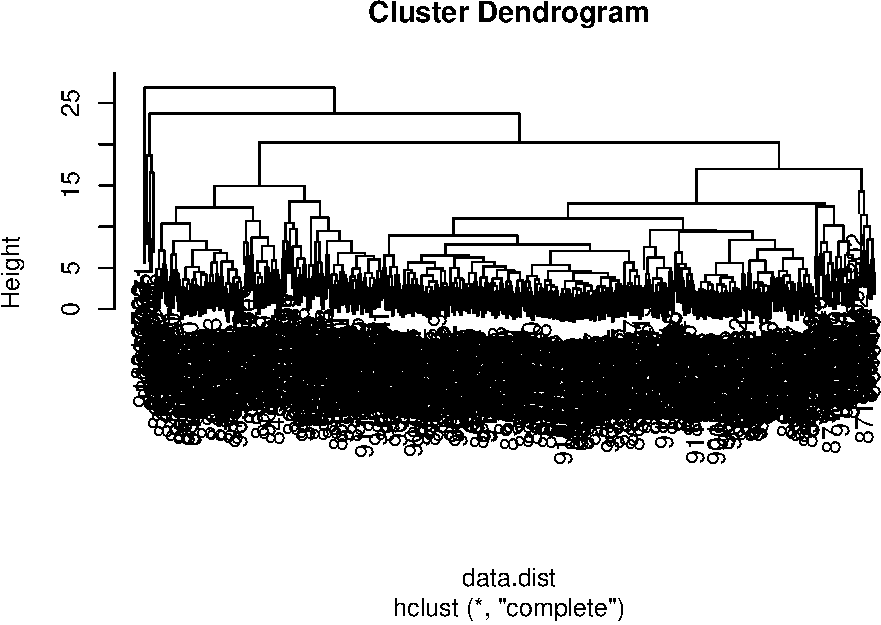
\includegraphics{lecture9_lab_files/figure-latex/tree_dummy-1.pdf}

\subsection{Selecting number of
clusters}\label{selecting-number-of-clusters}

In this section, you will compare the outputs from your hierarchical
clustering model to the actual diagnoses. Normally when performing
unsupervised learning like this, a target variable (i.e.~known answer or
labels) isn't available. We do have it with this dataset, however, so it
can be used to check the performance of the clustering model.

When performing supervised learning - that is, when you're trying to
predict some target variable of interest and that target variable is
available in the original data - using clustering to create new features
may or may not improve the performance of the final model.

This exercise will help you determine if, in this case, hierarchical
clustering provides a promising new feature.

Use \texttt{cutree()} to cut the tree so that it has 4 clusters. Assign
the output to the variable \texttt{wisc.hclust.clusters}.

\begin{Shaded}
\begin{Highlighting}[]
\NormalTok{wisc.hclust.clusters <-}\StringTok{ }\NormalTok{___}
\end{Highlighting}
\end{Shaded}

We can use the \texttt{table()} function to compare the cluster
membership to the actual diagnoses.

\begin{Shaded}
\begin{Highlighting}[]
\KeywordTok{table}\NormalTok{(wisc.hclust.clusters, diagnosis)}
\end{Highlighting}
\end{Shaded}

\begin{verbatim}
##                     diagnosis
## wisc.hclust.clusters   0   1
##                    1  12 165
##                    2   2   5
##                    3 343  40
##                    4   0   2
\end{verbatim}

Here we picked four clusters and see that cluster 1 largely corresponds
to malignant cells (with \texttt{diagnosis} values of 1) whilst cluster
3 largely corresponds to benign cells (with \texttt{diagnosis} values of
0).

Before moving on, explore how different numbers of clusters affect the
ability of the hierarchical clustering to separate the different
diagnoses.

\begin{itemize}
\tightlist
\item
  \textbf{Q12.} Can you find a better cluster vs diagnoses match with by
  cutting into a different number of clusters between 2 and 10?
\end{itemize}

\section{Section 4.}\label{section-4.}

\subsection{K-means clustering and comparing
results}\label{k-means-clustering-and-comparing-results}

As you now know, there are two main types of clustering: hierarchical
and k-means.

In this section, you will create a k-means clustering model on the
Wisconsin breast cancer data and compare the results to the actual
diagnoses and the results of your hierarchical clustering model. Take
some time to see how each clustering model performs in terms of
separating the two diagnoses and how the clustering models compare to
each other.

Create a k-means model on \texttt{wisc.data}, assigning the result to
\texttt{wisc.km}. Be sure to create 2 clusters, corresponding to the
actual number of diagnosis. Also, remember to scale the data (with the
\texttt{scale()} function and repeat the algorithm 20 times (by setting
setting the value of the \texttt{nstart} argument appropriately).
Running multiple times such as this will help to find a well performing
model.

\begin{Shaded}
\begin{Highlighting}[]
\NormalTok{wisc.km <-}\StringTok{ }\KeywordTok{kmeans}\NormalTok{(___, }\DataTypeTok{centers=}\NormalTok{ ___, }\DataTypeTok{nstart=}\NormalTok{ ___)}
\end{Highlighting}
\end{Shaded}

Use the \texttt{table()} function to compare the cluster membership of
the k-means model (\texttt{wisc.km\$cluster}) to the actual diagnoses
contained in the \texttt{diagnosis} vector.

\begin{Shaded}
\begin{Highlighting}[]
\KeywordTok{table}\NormalTok{(___, ___)}
\end{Highlighting}
\end{Shaded}

\begin{itemize}
\tightlist
\item
  \textbf{Q13}. How well does k-means separate the two diagnoses? How
  does it compare to your hclust results?
\end{itemize}

Use the table() function to compare the cluster membership of the
k-means model (\texttt{wisc.km\$cluster}) to your hierarchical
clustering model from above (\texttt{wisc.hclust.clusters}). Recall the
cluster membership of the hierarchical clustering model is contained in
\texttt{wisc.hclust.clusters} object.

\begin{Shaded}
\begin{Highlighting}[]
\KeywordTok{table}\NormalTok{(___, ___)}
\end{Highlighting}
\end{Shaded}

\begin{verbatim}
##                     
## wisc.hclust.clusters   1   2
##                    1 160  17
##                    2   7   0
##                    3  20 363
##                    4   2   0
\end{verbatim}

Looking at the second table you generated, it looks like clusters 1, 2,
and 4 from the hierarchical clustering model can be interpreted as the
cluster 1 equivalent from the k-means algorithm, and cluster 3 can be
interpreted as the cluster 2 equivalent.

\section{Section 5.}\label{section-5.}

\subsection{Clustering on PCA results}\label{clustering-on-pca-results}

In this final section, you will put together several steps you used
earlier and, in doing so, you will experience some of the creativity and
open endedness that is typical in unsupervised learning.

Recall from earlier sections that the PCA model required significantly
fewer features to describe 70\%, 80\% and 95\% of the variability of the
data. In addition to normalizing data and potentially avoiding
over-fitting, PCA also uncorrelates the variables, sometimes improving
the performance of other modeling techniques.

Let's see if PCA improves or degrades the performance of hierarchical
clustering.

Using the minimum number of principal components required to describe at
least 90\% of the variability in the data, create a hierarchical
clustering model with complete linkage. Assign the results to
\texttt{wisc.pr.hclust}.

\begin{Shaded}
\begin{Highlighting}[]
\NormalTok{## Use the distance along the first 7 PCs for clustering i.e. wisc.pr$x[, 1:7]}
\NormalTok{wisc.pr.hclust <-}\StringTok{ }\KeywordTok{hclust}\NormalTok{(___, }\DataTypeTok{method=}\NormalTok{___)}
\end{Highlighting}
\end{Shaded}

Cut this hierarchical clustering model into 4 clusters and assign the
results to \texttt{wisc.pr.hclust.clusters}.

\begin{Shaded}
\begin{Highlighting}[]
\NormalTok{wisc.pr.hclust.clusters <-}\StringTok{ }\KeywordTok{cutree}\NormalTok{(wisc.pr.hclust, }\DataTypeTok{k=}\DecValTok{4}\NormalTok{)}
\end{Highlighting}
\end{Shaded}

Using \texttt{table()}, compare the results from your new hierarchical
clustering model with the actual diagnoses.

\begin{itemize}
\tightlist
\item
  \textbf{Q14}. How well does the newly created model with four clusters
  separate out the two diagnoses?
\end{itemize}

\begin{Shaded}
\begin{Highlighting}[]
\CommentTok{# Compare to actual diagnoses}
\KeywordTok{table}\NormalTok{(___, diagnosis)}
\end{Highlighting}
\end{Shaded}

\begin{verbatim}
##                        diagnosis
## wisc.pr.hclust.clusters   0   1
##                       1   5 113
##                       2 350  97
##                       3   2   0
##                       4   0   2
\end{verbatim}

\begin{itemize}
\tightlist
\item
  \textbf{Q15}. How well do the k-means and hierarchical clustering
  models you created in previous sections (i.e.~before PCA) do in terms
  of separating the diagnoses? Again, use the \texttt{table()} function
  to compare the output of each model (\texttt{wisc.km\$cluster} and
  \texttt{wisc.hclust.clusters}) with the vector containing the actual
  diagnoses.
\end{itemize}

\begin{Shaded}
\begin{Highlighting}[]
\KeywordTok{table}\NormalTok{(___, diagnosis)}
\KeywordTok{table}\NormalTok{(___, diagnosis)}
\end{Highlighting}
\end{Shaded}

\begin{verbatim}
##    diagnosis
##       0   1
##   1  14 175
##   2 343  37
\end{verbatim}

\begin{verbatim}
##                     diagnosis
## wisc.hclust.clusters   0   1
##                    1  12 165
##                    2   2   5
##                    3 343  40
##                    4   0   2
\end{verbatim}

\section{Section 6.}\label{section-6.}

Sensitivity refers to a test's ability to correctly detect ill patients
who do have the condition. In our example here the sensitivity is the
total number of samples in the cluster identified as predominantly
malignant (cancerous) divided by the total number of known malignant
samples.

Specificity relates to a test's ability to correctly reject healthy
patients without a condition. In our example specificity is the
proportion of benign (not cancerous) samples in the cluster identified
as predominantly benign that are known to be benign.

\begin{itemize}
\tightlist
\item
  \textbf{Q16.} Which of your analysis procedures resulted in a
  clustering model with the best specificity? How about sensitivity?
\end{itemize}

\section{Section 7.}\label{section-7.}

\subsection{PCA of protein structure
data}\label{pca-of-protein-structure-data}

Visit the Bio3D-web PCA app \textless{} \url{http://bio3d.ucsd.edu}
\textgreater{} and explore how PCA of large protein structure sets can
provide considerable insight into major features and trends with clear
biological mechanistic insight. Note that the final report generated
from this app contains all the R code required to run the analysis
yourself - including PCA and clustering. We will delve more into this
type of analysis in the next class.

\section{About this document}\label{about-this-document}

This is an \href{http://rmarkdown.rstudio.com}{R Markdown} Notebook.
When you execute code within the notebook, the results appear beneath
the code.

Try executing any code chunk by clicking the \emph{Run} button within
the chunk or by placing your cursor inside it and pressing
\emph{Cmd+Shift+Enter}.

Add a new chunk by clicking the \emph{Insert Chunk} button on the
toolbar or by pressing \emph{Cmd+Option+I}.

When you save the notebook, an HTML file containing the code and output
will be saved alongside it (click the \emph{Preview} button or press
\emph{Cmd+Shift+K} to preview the HTML file).

The preview shows you a rendered HTML copy of the contents of the
editor. Consequently, unlike \emph{Knit}, \emph{Preview} does not run
any R code chunks. Instead, the output of the chunk when it was last run
in the editor is displayed.

Here we use the \texttt{sessionInfo()} function to report on our R
systems setup at the time of document execution.

\begin{Shaded}
\begin{Highlighting}[]
\KeywordTok{sessionInfo}\NormalTok{()}
\end{Highlighting}
\end{Shaded}

\begin{verbatim}
## R version 3.4.1 (2017-06-30)
## Platform: x86_64-apple-darwin15.6.0 (64-bit)
## Running under: macOS Sierra 10.12.6
## 
## Matrix products: default
## BLAS: /Library/Frameworks/R.framework/Versions/3.4/Resources/lib/libRblas.0.dylib
## LAPACK: /Library/Frameworks/R.framework/Versions/3.4/Resources/lib/libRlapack.dylib
## 
## locale:
## [1] en_US.UTF-8/en_US.UTF-8/en_US.UTF-8/C/en_US.UTF-8/en_US.UTF-8
## 
## attached base packages:
## [1] stats     graphics  grDevices utils     datasets  methods   base     
## 
## loaded via a namespace (and not attached):
##  [1] compiler_3.4.1  backports_1.1.2 magrittr_1.5    rprojroot_1.3-2
##  [5] tools_3.4.1     htmltools_0.3.6 yaml_2.1.16     Rcpp_0.12.14   
##  [9] stringi_1.1.6   rmarkdown_1.8   knitr_1.18      stringr_1.2.0  
## [13] digest_0.6.14   evaluate_0.10.1
\end{verbatim}


\end{document}
